% !TEX program = xelatex
\documentclass[fontsize=14pt,a4paper]{scrartcl}
\usepackage[english,russian]{babel} 
\usepackage{fontspec} 
\defaultfontfeatures{Ligatures={TeX},Renderer=Basic} 
\setmainfont[Ligatures=TeX]{PT Astra Serif}

\usepackage{unicode-math}
\unimathsetup{math-style=TeX}
\setmathfont{Cambria Math}
\setmathfont[range=\mathup/{num}]{PT Astra Serif}
\setmathfont[range=\mathit/{greek,Greek,latin,Latin,Cyrillic,cyrillic}]{Cambria Math}
\setmathfont[range=\mathup/{greek,Greek,latin,Latin,Cyrillic,cyrillic}]{Cambria Math}
\setmathfont[range={"2212,"002B,"003D,"0028,"0029,"005B,
"005D,"221A,"2211,"2248,"222B,"007C,"2026,"2202,"00D7,"0302,
"2261,"0025,"22C5,"00B1,"2194,"21D4}]{Cambria Math}

\usepackage{indentfirst}
\usepackage{graphicx}
\usepackage{amsmath}

\usepackage{pgfplots}
\usepackage{pgfplotstable}

\def\arraystretch{1.3}%

\usepackage[left=20mm, top=20mm, right=10mm, bottom=20mm, nohead, footskip=10mm]{geometry}
\begin{document}
  \begin{titlepage}                                                         
    \newpage                                                                        
    \begin{center}   
      Министерство образования и науки Российской Федерации  \\ 
      \vspace{1em}                                                    
      {\mdseries
        Федеральное государственное бюджетное образовательное \\
        учреждение высшего образования \\
        «ОМСКИЙ ГОСУДАРСТВЕННЫЙ ТЕХНИЧЕСКИЙ УНИВЕРСИТЕТ»
      }                               
      \vspace{1em}      

      {\bfseries Кафедра «Средства связи и информационная безопасность»}  

      \vspace{\fill}                                                         
                                   
      {\bfseries ОТЧЕТ } \\                                 
      По дисциплине «Электродинамика и распространение радиоволн» \\ 
      \vspace{1em} 
      Практическая работа №3 \\                                                           
    \end{center}                                                          
                                                                                        
    \vspace{\fill}                                                         
                                                                                        
    \hfill\parbox{5cm}{
      Выполнил\\
      студент гр. ЗИС-231:\\
      Белый В.Е. \\
      \\
      Проверил:\\
      проф., д.н. \\
      Богачков И.В.\\
    }                                                                                                                              
                                                                                                                                                                              
    \vspace{\fill}                                                    
                                                                                        
    \begin{center}                                                        
    Омск, 2026                                                                
    \end{center}                                                          
                                                                                        
    \end{titlepage}

    \newpage
    {\bfseries Задание 3.} 
    Плоская ЭМВ (поляризация неизвестна) наклонно падает из диэлектрика с параметрами $ \varepsilon $ (табл. 1), $\mu=1$, $\sigma=1$ на плоскую границу раздела с вакуумом.
    \\ \indent Рассчитать значение критического угла и угла Брюстера. Описать условия полного отражения и полного прохождения.
    \\ \indent Построить графики зависимостей модулей коэффициентов отражения $\left(\lvert \textup{Г}(φ)\lvert\right)$ и преломления $\left(\lvert \textup{T}(φ)\lvert\right)$ от угла падения $\left(\varphi=0…90^{\circ}\right)$.    

    \begin{table}[ht!]
      \begin{center}
        \label{tab:table1}
        \begin{tabular}{|l|l|}
          \hline
          Вариант & $\varepsilon$   \\
          \hline
          $45$    & $4,4$           \\
          \hline
        \end{tabular}
        \caption{Исходные данные.}
      \end{center}
    \end{table}

    {\bfseries Решение:} 
    \\ \indent В случае, когда ЭМВ падает из оптически более плотной среды в менее плотную, возникает явление полного отражения, если угол падения превышает критический угол. Если угол падения больше критического, то отраженная волна уносит всю энергию, принесенную падающей ЭМВ. При угле Брюстера коэффициент отражения превращается в ноль, ЭМВ полностью переходит во вторую среду.
    \\ \indent Рассчитываем значение критического угла и угла Брюстера, при котором отраженная волна отсутствует:
    \[\varepsilon_1 = 4,4, \; \varepsilon_2 = 1\]
    \begin{equation} \varphi_{\textup{Бр}} = arctg\sqrt{\frac{\varepsilon_2}{\varepsilon_1}}, \; \varphi_{\textup{Бр}} = 25,49^{\circ}; \end{equation}
    \begin{equation} \varphi_{\textup{кр}} = arcsin{\sqrt{\frac{\varepsilon_2\cdot\mu_2}{\varepsilon_1\cdot\mu_1}}}, \; \varphi_{\textup{кр}} = 28,47^{\circ}; \end{equation}

    Рассчитаем углы преломления, описанные законом Снеллиуса: \\

    \begin{equation} \frac{\sin\varphi}{\sin\psi}=\frac{\sqrt{\varepsilon_2}}{\sqrt{\varepsilon_1}}, \; \psi = arcsin\left(\frac{\sin\varphi\cdot\sqrt{\varepsilon_1}}{\sqrt{\varepsilon_2}}\right);\end{equation}

    \newpage
    Рассчитаем значения коэффициентов отражения и преломления для перпендикулярной и параллельной поляризации:\\

    \begin{equation} \textup{Г}_{\perp} = \frac{\sin(\psi-\varphi)}{\sin(\psi+\varphi)}, \; \textup{Г}_{\parallel} = \frac{\tg(\psi-\varphi)}{\tg(\psi+\varphi)}; \end{equation}
    \begin{equation} \textup{Т}_{\perp} = \frac{2\cdot\sin\psi\cdot\cos\varphi}{\sin(\psi+\varphi)}, \; \textup{Т}_{\parallel} = \frac{2\cdot\sin\psi\cdot\cos\varphi}{\sin{\left(\psi+\varphi\right)}\cdot\cos(\psi-\varphi)}; \end{equation}

    \vspace{\fill}

    \begin{table}[h]
    \begin{center}
      \label{tab:table2}
      \pgfplotstabletypeset[
        column type=l,
        before row=\hline,every last row/.style={after row=\hline},
        columns/fi/.style={
          column type=|l|,
          column name={$\varphi$},
        },
        columns/psi/.style={
          column type=l|,
          column name={$\psi$},
        },
        columns/G1/.style={
          column type=l|,
          column name={$\textup{Г}_{\perp}$},
        },
        columns/G2/.style={
          column type=l|,
          column name={$\textup{Г}_{\parallel}$},
        },
        columns/T1/.style={
          column type=l|,
          column name={$\textup{Т}_{\perp}$},
        },
        columns/T2/.style={
          column type=l|,
          column name={$\textup{Т}_{\parallel}$},
        },
        col sep=semicolon,
        /pgf/number format/read comma as period
      ]{data/data.csv}
      \caption{Коэффициенты отражения и преломления для перпендику­лярной и параллельной поляризации.}
    \end{center} 
    \end{table}
    
    \vspace{\fill}

    \newpage
    Построим графики зависимостей модулей коэффициентов отражения $\left(\lvert \textup{Г}(\varphi)\lvert\right)$ и преломления $\left(\lvert \textup{T}(\varphi)\lvert\right)$: \\
    
    \begin{center}

      \begin{figure}[h!]
        \centering
        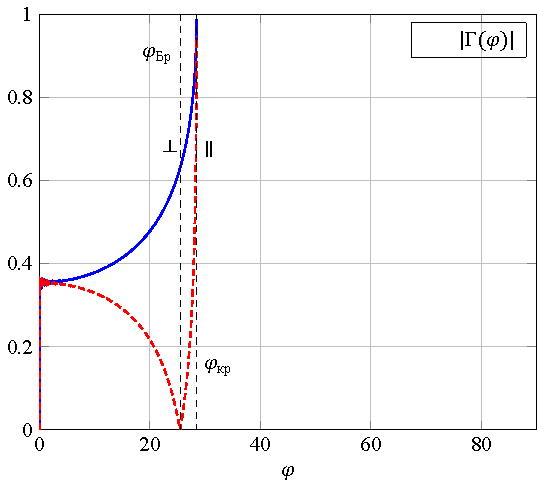
\includegraphics[scale=1]{data/fig/Г}
        \caption{График зависимостей модулей коэффициентов отражения}
        \label{fig:ris1}
      \end{figure}

      \begin{figure}[h!]
        \centering
        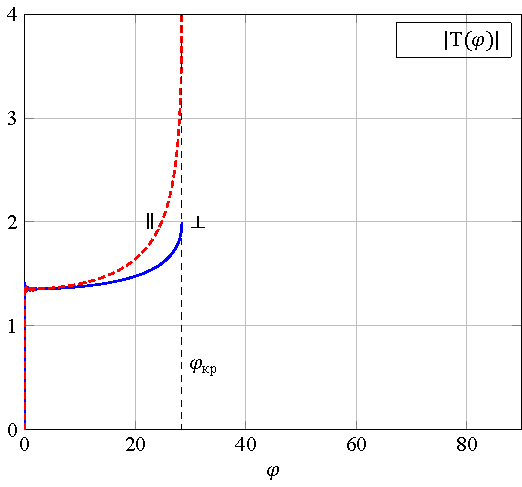
\includegraphics[scale=1]{data/fig/Т}
        \caption{График зависимостей модулей коэффициентов преломления}
        \label{fig:ris2}
      \end{figure}

    \end{center}
\end{document}